\begin{frame}{Raspbian-Info}
	\begin{itemize}
		\item Version of Debian(Linux) optimized for RPi
		\item Linux commands run
		\item Shell
		\begin{itemize}
			\item Command line interface between OS and user
			\item Many shells exist
			\item We will use BASH (Bourne Again SHell)
			\item BASH is default shell for Raspbian
		\end{itemize}
		\item Console/Terminal
		\begin{itemize}
			\item Text entry and display device
			\item can be physical device
			\item Now one mostly uses virtual terminal
			\begin{itemize}
				\item A software emulator of terminal
			\end{itemize}
			\item LXTerminal is default terminal in Raspbian
			\item Prompt is \$
		\end{itemize}
	\end{itemize}
\end{frame}

\begin{frame}{Raspbian-login}
	\begin{itemize}
		\item User Accounts
		\begin{itemize}
			\item Linux Machine can entertain multiple user accounts at same time
			\item Each account is access using a \textbf{username} and a \textbf{password}
			\item Process of accessing a machine using an account is called \textbf{login}
			\item Default:
			\begin{itemize}
				\item username = pi
				\item password = raspberry
			\end{itemize}
		\end{itemize}
	\end{itemize}
\end{frame}

\begin{frame}{Raspbian-file system}
	\begin{figure}
		\centering
		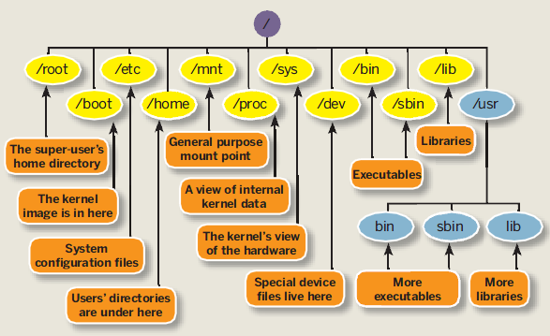
\includegraphics[width=8.5cm,height=8.5cm,keepaspectratio]{linux_filesystem}
		\caption{Linux file system}
	\end{figure}
	Ref: \url{http://www.siongboon.com/projects/2013-07-08_raspberry_pi/images/linux_filesystem.png}
\end{frame}
\begin{frame}{Traversing raspbian file structure}
	\begin{itemize}
		\item \textbf{pwd} = print working directory
		\item \textbf{mkdir} = make directory
		\item \textbf{rmdir} = remove directory
		\item \textbf{rmdir -r} = remove directory recursively
		\item \textbf{cd} = change directory
		\item \textbf{cd ..} = step back in directory by one step
		\item \textbf{/} = step back to home
		\item \textbf{ls} = lists the contents of directory
		\item \textbf{ls -l} = long list of contents with great details
	\end{itemize}
\end{frame}

\begin{frame}{Text Editors}
	\begin{itemize}
		\item For creating and modifying a file
		\item A word processors but simpler
		\item Two types:
		\begin{itemize}
			\item Command line based
			\begin{itemize}
				\item emacs, vi, vim, nano
			\end{itemize}
			\item GUI based
			\begin{itemize}
				\item gedit
			\end{itemize}
		\end{itemize}
	\end{itemize}
\end{frame}

\begin{frame}{Making and Viewing Files}
	\begin{itemize}
		\item Write the name of text editor succeeded by file
		\item If a file does not exist, it is created and opened for editing
		\begin{itemize}
			\item \textbf{nano test.py}
		\end{itemize}
		\item \textbf{cat test} prints the file to the terminal
		\item \textbf{head test} prints the first $10$ lines
		\item \textbf{last test} or \textbf{tail test} prints last $10$ lines
		\item \textbf{cp test new-test} copes file \textbf{test} to a new file \textbf{new-test}
		\item \textbf{mv test a/test1} moves \textbf{test} file to a new destination (/a/) by \textit{renaming} it \textbf{test1}
		\item \textcolor{blue}{create a file, view and edit the contents, make a copy and delete the copy and then rename it!}
	\end{itemize}
\end{frame}

\begin{frame}{Permission}
	\begin{itemize}
		\item Files has owner (user) and defined permission
		\begin{itemize}
			\item read (r)
			\item write (w)
			\item execute (x)
		\end{itemize} 
		\item Permission are assigned according to type:
		\begin{itemize}
			\item user : file owner
			\item group : a permission group
			\item other : all users
		\end{itemize}
		\item Type \textbf{ls -l} to see these permissions
		\item Do this at home directory
		\item For \textbf{Desktop} directory it shows following permission
		\begin{itemize}
			\item \textbf{drwxr-xr-x}
			\item \textbf{d} shows that its a directory
			\item Next three symbols define \textit{user} permissions \textbf{rwr}
			\item Next three symbols define \textit{group} permissions \textbf{r-x}
			\item Next three symbols define \textit{other} permissons \textbf{r-x}
		\end{itemize}
		\item \textcolor{blue}{create a file and check out its permissions}
	\end{itemize}
\end{frame}

\begin{frame}{Root}
	\begin{itemize}
		\item Root account has highest permission level
		\item Key files and directory is accessible only to root
		\item Sometimes you would need to be root
		\begin{itemize}
			\item To install a program
			\item Change OS as per requirements
		\end{itemize}
		\item \textbf{su} : super-user
		\begin{itemize}
			\item asks for root password
			\item If password is correct, one login as root
		\end{itemize}
		\item \textbf{sudo}: super-user do
		\begin{itemize}
			\item Just applies root permission for single command
			\item Ex: \textbf{sudo ls} will simply apply root permission for listing the files
			\item safer way!
		\end{itemize}
	\end{itemize}
\end{frame}

\begin{frame}{Processes}
	\begin{itemize}
		\item A process is an executing of program
		\item Processes can run in two ways:
		\begin{itemize}
			\item foreground
			\item background (demons)
		\end{itemize}
		\item type \textbf{ps a} to see all processes
		\item All processes are associated with a unique ID (an integer number)
		\item This number can be used to control the process
		\begin{itemize}
			\item \textbf{kill} can be used to end a process
		\end{itemize}
		\item \textbf{shutdown} command shutdowns a Linux machine properly
	\end{itemize}
\end{frame}